\documentclass[aspectratio=169,14pt]{beamer}
\usepackage{graphicx}
\usepackage[export]{adjustbox} % allows valign option
\usepackage{mathtools} % for xmapsto

% remove all navigation symbols
\setbeamertemplate{navigation symbols}{}

% remove headline and footline
\setbeamertemplate{headline}{}
\setbeamertemplate{footline}{}

% ensure plain white background
\setbeamertemplate{background canvas}{\color{white}\rule{\paperwidth}{\paperheight}}

\usepackage{tikz}
\usetikzlibrary{knots,hobby,decorations.markings}
\usetikzlibrary {arrows.meta,bending,positioning}

%\usecolortheme{whale}

\title{\Huge Knot Theory}
\author{\Large Jim Fowler (\texttt{@kisonecat})}
\date{May 1, 2025 = $(1+2+\cdots+8+9)^2 = 1^3 + 2^3 + \cdots + 8^3 + 9^3$}

\newcommand{\fullpageslideblack}[1]{%
  \begin{frame}[plain]
    \begin{tikzpicture}[remember picture,overlay]
      % black background
      \fill[black] (current page.south west) rectangle (current page.north east);
      % full‐page image (keeps aspect ratio)
      \node[anchor=center] at (current page.center)
        {\includegraphics[width=\paperwidth,height=\paperheight,keepaspectratio]{#1}};
    \end{tikzpicture}
  \end{frame}
}

\newcommand{\fullpageslidewhite}[1]{%
  \begin{frame}[plain]
    \begin{tikzpicture}[remember picture,overlay]
      % black background
      \fill[white] (current page.south west) rectangle (current page.north east);
      % full‐page image (keeps aspect ratio)
      \node[anchor=center] at (current page.center)
        {\includegraphics[width=\paperwidth,height=\paperheight,keepaspectratio]{#1}};
    \end{tikzpicture}
  \end{frame}
}

\newcommand{\tangleT}{
  \begin{scope}
    % The central square
    \draw[fill=white!90!black] (-1,-1) rectangle (1,1);
    
    % Label T at the center
    \node at (0,0) {tangle};
  \end{scope}
}

\newcommand{\tanglerotate}[1]{
  \begin{scope}[rotate=90,transform shape]
    #1
  \end{scope}
}

\newcommand{\tangleshrinktwist}[1]{
  \begin{scope}[xshift=-0.25cm]
    \begin{scope}[scale=0.5,transform shape]
      #1
    \end{scope}
  \end{scope}
  
  % Four strands from the corners
  \draw (-0.75, 0.5) to[out=135,in=-45] (-1,1);
  \draw (-0.75,-0.5) to[out=225,in=45] (-1,-1);
  
  \begin{knot}[clip width=4,clip radius=6pt,ignore endpoint intersections=false]
    \strand ( 0.25, 0.5) to[out=45,in=135] ( 1,-1);
    \strand ( 0.25,-0.5) to[out=-45,in=-135] ( 1,1);
  \end{knot}    
}

\newcommand{\tangletwist}[1]{
  \begin{scope}[xshift=-0.5cm]
    \begin{scope}[xscale=0.5,transform shape]
      #1
    \end{scope}
  \end{scope}
  
  \begin{knot}[clip width=4,clip radius=6pt,ignore endpoint intersections=false]
    \strand ( 0, 1) to[out=45,in=135] ( 1,-1);
    \strand ( 0,-1) to[out=-45,in=-135] ( 1,1);
  \end{knot}    
}

\newcommand{\tanglezero}{
  \begin{knot}[clip width=4,clip radius=6pt,ignore endpoint intersections=false]
    \strand ( -1, 1) to[out=-45,in=225] ( 1,1);
    \strand ( -1,-1) to[out=45,in=-225] ( 1,-1);
  \end{knot}    
}

\newcommand{\tangleinfty}{\tanglerotate{\tanglezero}}

\newcommand{\tangleone}{
  \begin{knot}[clip width=4,clip radius=6pt,ignore endpoint intersections=false]
    \strand ( -1, 1) to[out=-45,in=-225] (0,0) to[out=-45,in=-225] ( 1,-1);
    \strand ( -1,-1) to[out=45,in=225] (0,0)  to[out=45,in=225] ( 1,1);
  \end{knot}    
}

\newcommand{\displaytangle}[1]{
  \begin{tikzpicture}[line width=1pt]
    % \tangletwist{\tanglerotate{\tangletwist{\tangletwist{\tangleT}}}}
    % \tangletwist{\tangletwist{\tangleone}}
    % \tangletwist{\tangleT}
    #1
    
    \draw (-1,-1) -- (-1.5,-1.5);
    \draw ( 1,-1) -- ( 1.5,-1.5);
    \draw (-1, 1) -- (-1.5, 1.5);
    \draw ( 1, 1) -- ( 1.5, 1.5);
    
    \draw[dotted] (0,0) circle (2.12132034355964);
  \end{tikzpicture}
}

\begin{document}

\frame{\titlepage}

\begin{frame}
  \begin{center}
    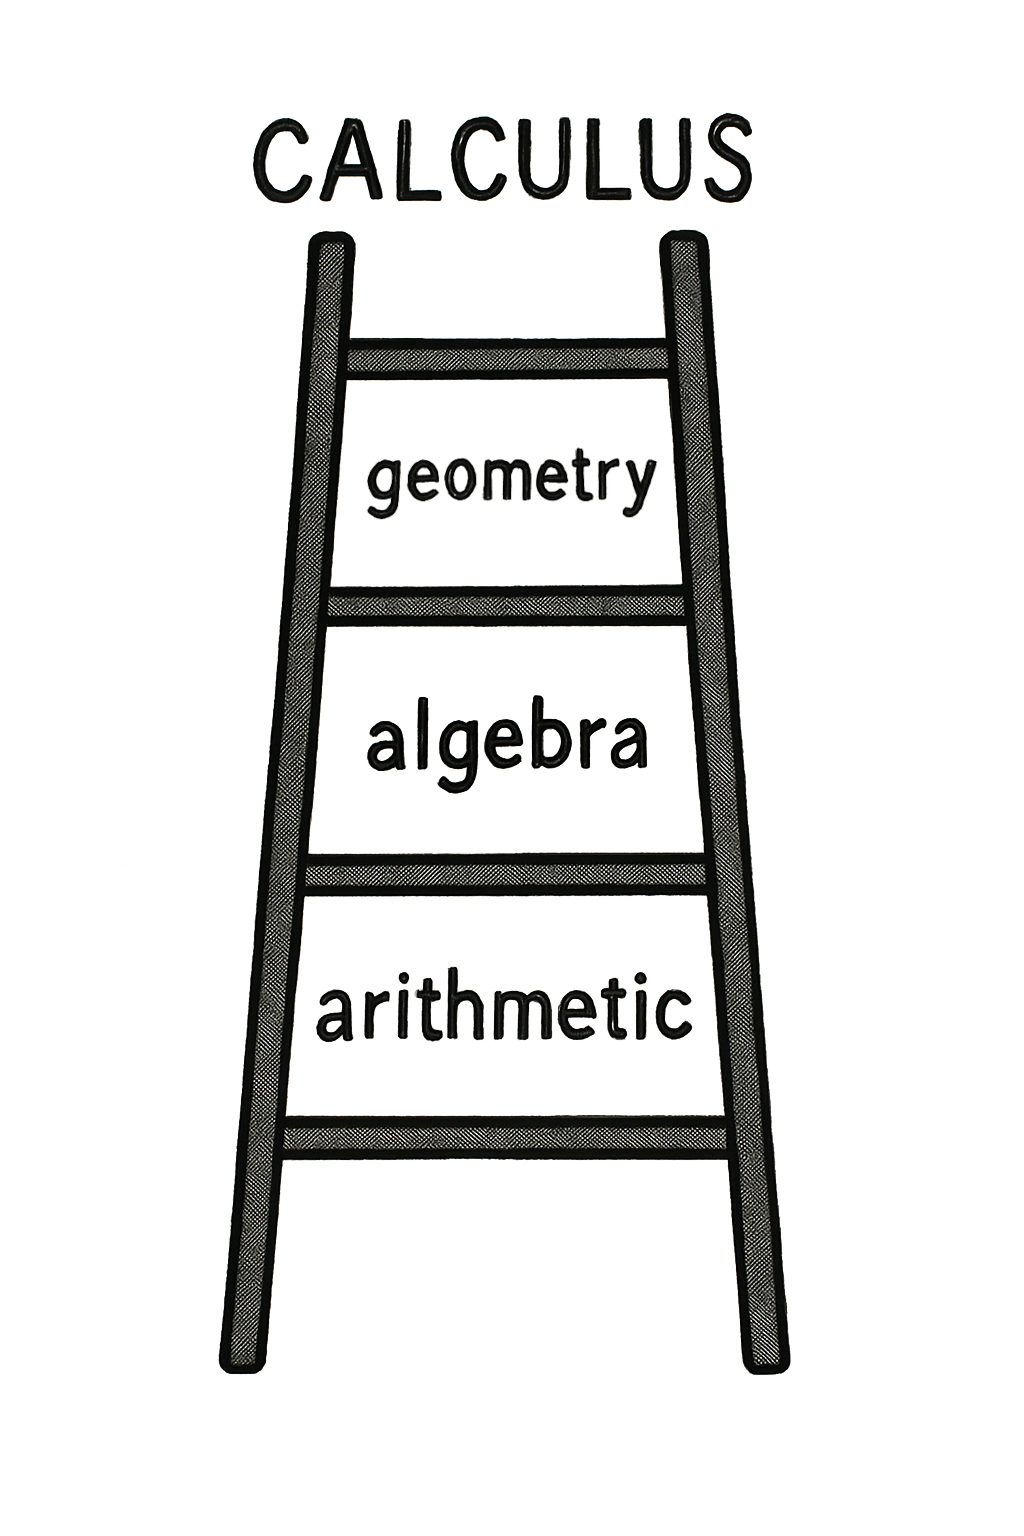
\includegraphics[height=\paperheight]{ladder-of-math.png}
  \end{center}
\end{frame}

\begin{frame}
  \begin{center}
    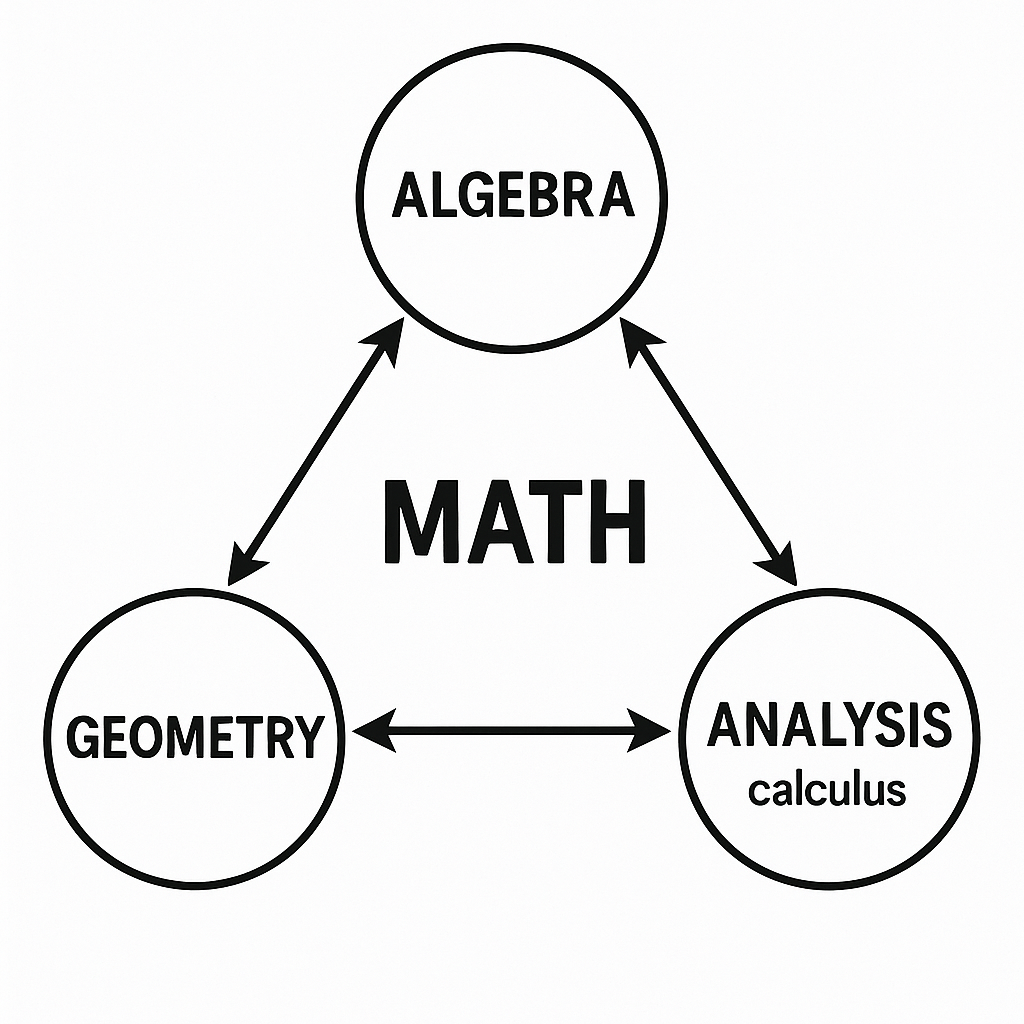
\includegraphics[width=\paperheight]{math-as-triangle.png}
  \end{center}
\end{frame}

\begin{frame}
  \Large
  
  \begin{itemize}
  \item What's a knot?
  \item Are there nontrivial knots?
  \item How do knots relate to algebra?
  \end{itemize}
\end{frame}

\begin{frame}
  \frametitle{Real-life knots\ldots}
  \begin{center}
    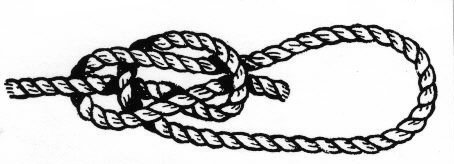
\includegraphics[width=5.8in]{bowline.jpg}
  \end{center}
\end{frame}

\fullpageslidewhite{wikipedia-knot.png}

\fullpageslidewhite{wikipedia-math-knot.png}

\begin{frame}
  \frametitle{Mathematical knots}

  \begin{columns}
    \begin{column}{0.4\paperwidth}
      \begin{center}
  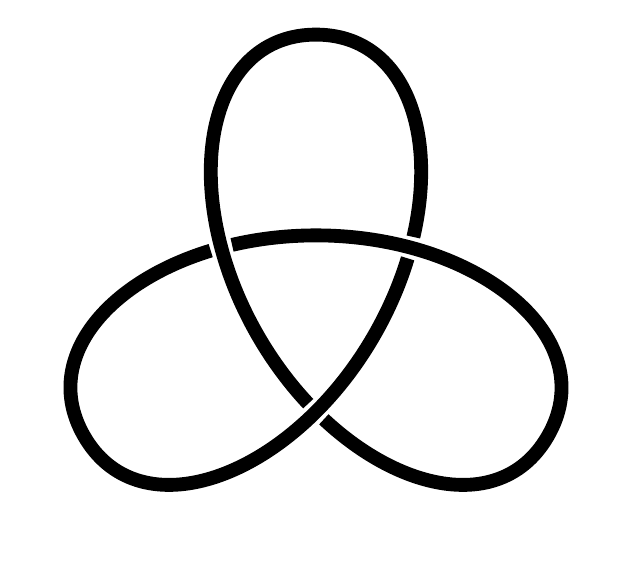
\begin{tikzpicture}[
    scale=1.7,
use Hobby shortcut,
every trefoil component/.style={ultra thick, draw, line width=5pt},
%trefoil component 1/.style={red},
%trefoil component 2/.style={blue},
%trefoil component 3/.style={green},
]
\path[spath/save=trefoil] ([closed]90:2) foreach \k in {1,...,3} {
.. (-30+\k*240:.5) .. (90+\k*240:2) } (90:2);
\tikzset{spath/knot={trefoil}{8pt}{1,3,5}}
\end{tikzpicture}
\end{center}
\end{column}
\begin{column}{0.54\paperwidth}
  \begin{center}
    \Large
    Knots are \textit{closed} \\
    ---no loose ends--- \\
    so a knot is a tied up circle!
  \end{center}
  \vspace{1in}
  \null
\end{column}
\end{columns}
\end{frame}

% examples of knots
\fullpageslidewhite{knots.pdf}

% TODO: different unknots

\begin{frame}
  \frametitle{Wiggle the diagram? Same knot.}
  \begin{center}
  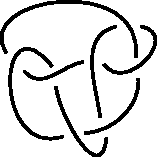
\includegraphics[width=1.5in]{knot-76.pdf} \hfill\raisebox{0.7in}{$=$}\hfill
  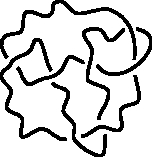
\includegraphics[width=1.5in]{knot-76-2.pdf} \hfill\raisebox{0.7in}{$=$}\hfill
  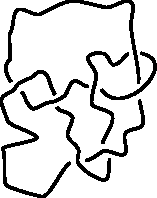
\includegraphics[width=1.5in]{knot-76-3.pdf}
  \end{center}
\end{frame}

\begin{frame}
  \frametitle{But wiggling isn't enough}
  
  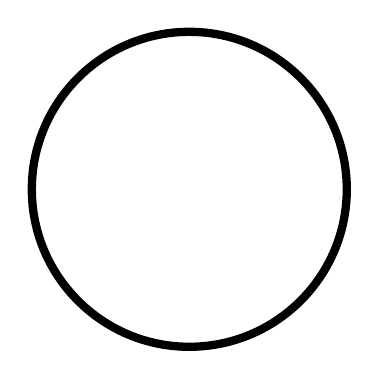
\begin{tikzpicture}[scale=2]
  \begin{knot}
    \strand[line width=3pt] (0,0) circle (1cm);
  \end{knot}
\end{tikzpicture}
\hfill\raisebox{2cm}{$=$}\hfill
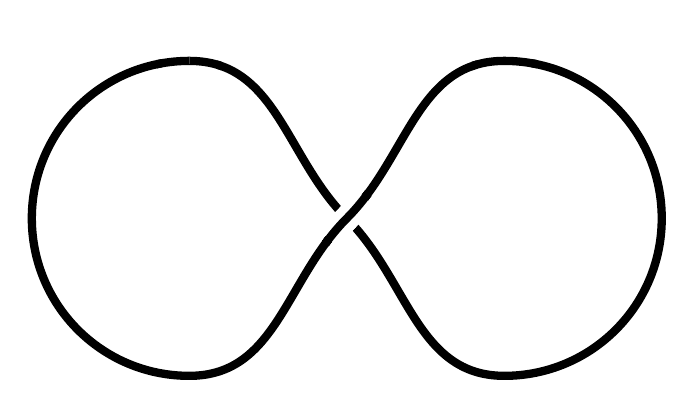
\begin{tikzpicture}[scale=2]
  \begin{knot}[
    clip width=3pt,               % how big the “gap” is at crossings
    consider self intersections,  % detect and break crossings automatically
    end tolerance=.001pt,
  ]
    \strand[line width=3pt]
    (-1,1) to[out=180, in=90]   (-2,0)
            to[out=270, in=180] (-1,-1)
            to [out=0,in=225] (0,0)
            to[out=45,  in=180] (1,1)
            to[out=0,   in=90]  (2,0)
            to[out=-90, in=0]   (1,-1)
            to[out=180, in=315] (0,0)
            to[out=135,  in=0]  cycle;
  \end{knot}
\end{tikzpicture}


\end{frame}

\tikzset{overcross/.style={double, line width=1.5, white, double=#1, double distance=\knotlinewidth},
    overcross/.default={black},
    knot/.style={line width=\knotlinewidth, baseline=-.5ex}}
\newcommand{\knotlinewidth}{.7pt}
\newcommand{\myarrow}{$\quad\longleftrightarrow\quad$}

%%%%%%%%%%%%%%%%%%%%%%%%%%%%%%%%%%%%%%%%%%%%%%%%%%%%%%%%%%%%%%%%
\begin{frame}
  \frametitle{Reidemeister Move I}

  \newcommand{\RIa}{\tikz[knot,yscale=1]{\draw(-.5,.5) to[out=-90,in=-90] (.5,0); \draw[overcross] (.5,0) to[out=90,in=90] (-.5,-.5);}}
\newcommand{\RIb}{\tikz[knot]{\draw[looseness=.8] (-.5,-.5) to[out=90, in=-90] (.5,0) to[out=90, in=-90] (-.5,.5);}}
  \newcommand{\RIc}{\tikz[knot,yscale=-1]{\draw(-.5,.5) to[out=-90,in=-90] (.5,0); \draw[overcross] (.5,0) to[out=90,in=90] (-.5,-.5);}}

\scalebox{2}{\RIa\myarrow\RIb\myarrow\RIc}

\end{frame}

%%%%%%%%%%%%%%%%%%%%%%%%%%%%%%%%%%%%%%%%%%%%%%%%%%%%%%%%%%%%%%%%
\begin{frame}
  \frametitle{Reidemeister Move II}

\newcommand{\RIIa}{\tikz[knot]{\draw[looseness=2.3] (-.5,-.5) to[out=0, in=0] (-.5,.5); \draw[looseness=2.3, overcross=black] (.5,-.5) to[out=180, in=180] (.5,.5);}}
  \newcommand{\RIIb}{\tikz[knot]{\draw[looseness=1.4] (-.5,-.5) to[out=0, in=0] (-.5,.5);\draw[looseness=1.4] (.5,.5) to[out=180,in=180] (.5,-.5);}}
  \newcommand{\RIIc}{\tikz[knot]{\draw[looseness=2.3] (.5,-.5) to[out=180,
      in=180] (.5,.5); \draw[looseness=2.3, overcross=black] (-.5,-.5) to[out=0,in=0] (-.5,.5);}}

  \begin{center}
\scalebox{2}{\RIIa\myarrow\RIIb\myarrow\RIIc}
\end{center}

\end{frame}


%%%%%%%%%%%%%%%%%%%%%%%%%%%%%%%%%%%%%%%%%%%%%%%%%%%%%%%%%%%%%%%%
\begin{frame}
  \frametitle{Reidemeister Move III}

\newcommand{\RIIIa}{\tikz[knot]{\draw (-120:.58) to[out=60,in=-120] (150:.2) to[out=60, in=-120] (60:.58); \draw[rotate=-120, overcross=black] (-120:.58) to[out=60, in=-120] (150:.2) to[out=60, in=-120] (60:.58); \draw[rotate=120, overcross=black] (-120:.58) to[out=60, in=-120] (150:.2) to[out=60, in=-120] (60:.58);}}

\newcommand{\RIIIb}{\tikz[knot, rotate=180]{\draw (-120:.58) to[out=60,in=-120] (150:.2) to[out=60, in=-120] (60:.58); \draw[rotate=-120, overcross=black] (-120:.58) to[out=60, in=-120] (150:.2) to[out=60, in=-120] (60:.58); \draw[rotate=120, overcross=black] (-120:.58) to[out=60, in=-120] (150:.2) to[out=60, in=-120] (60:.58);}}

\newcommand{\RIIIc}{\tikz[knot, xscale=-1]{\draw (-120:.58) to[out=60,in=-120] (150:.2) to[out=60, in=-120] (60:.58); \draw[rotate=-120, overcross=black] (-120:.58) to[out=60, in=-120] (150:.2) to[out=60, in=-120] (60:.58); \draw[rotate=120, overcross=black] (-120:.58) to[out=60, in=-120] (150:.2) to[out=60, in=-120] (60:.58);}}

\newcommand{\RIIId}{\tikz[knot, xscale=-1, rotate=180]{\draw (-120:.58) to[out=60,in=-120] (150:.2) to[out=60, in=-120] (60:.58); \draw[rotate=-120, overcross=black] (-120:.58) to[out=60, in=-120] (150:.2) to[out=60, in=-120] (60:.58); \draw[rotate=120, overcross=black] (-120:.58) to[out=60, in=-120] (150:.2) to[out=60, in=-120] (60:.58);}}

\begin{center}
\scalebox{2.5}{\RIIIa\myarrow\RIIIb}
\end{center}

\vfill

\begin{center}
\scalebox{2.5}{\RIIId\myarrow\RIIIc}
\end{center}

\end{frame}


\begin{frame}
  
  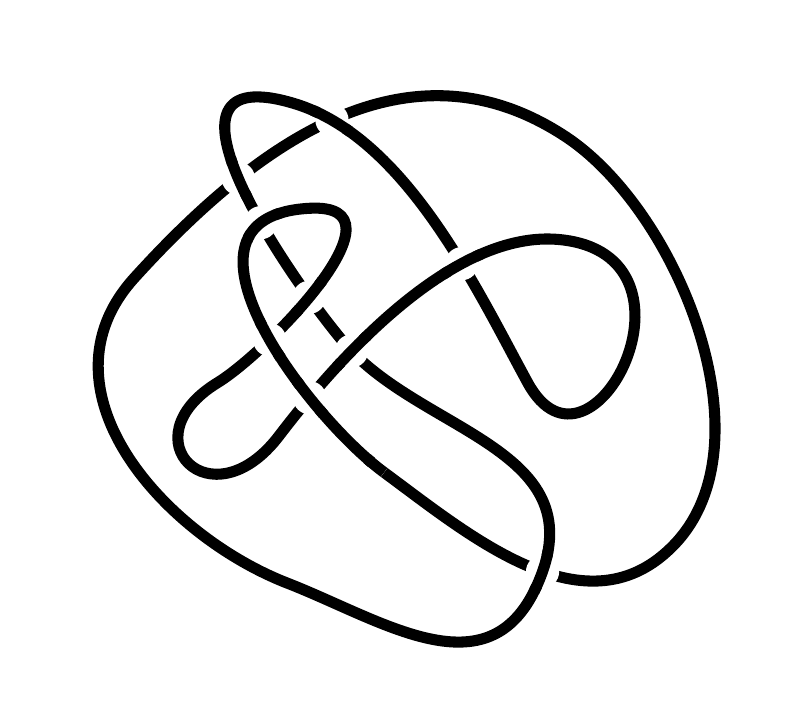
\begin{tikzpicture}[yscale=0.4,xscale=0.4]
    \begin{knot}[clip width=5pt,clip radius=6pt,ignore endpoint intersections=false,consider self intersections]
      %end tolerance=.001pt,
  \strand[line width=4pt] (10.3621, 15.1163).. controls (7.9553, 16.8877) and (3.0853, 23.2447) .. (8.0017, 23.5013).. controls (11.3053, 23.6736) and (6.6281, 18.9098) .. (5.0805, 17.9665).. controls (2.1878, 16.2035) and (4.866, 13.441) .. (7.0286, 16.2761).. controls (8.9843, 18.8399) and (12.5938, 22.8264) .. (15.9296, 22.5082).. controls (20.8911, 22.0348) and (16.9404, 14.2718) .. (14.9244, 17.9616).. controls (13.3204, 20.8975) and (11.0582, 25.7601) .. (7.5067, 26.8284).. controls (2.5077, 28.3322) and (7.3351, 21.3197) .. (9.0895, 19.2365).. controls (11.5124, 16.3594) and (17.1971, 15.876) .. (15.206, 11.5018).. controls (13.6591, 8.1033) and (10.3137, 10.4225) .. (7.2921, 11.5995).. controls (3.3656, 13.1291) and (-0.7768, 17.7474) .. (2.434, 21.2904).. controls (6.3124, 25.5701) and (11.1312, 29.06) .. (16.1149, 25.7838).. controls (19.6827, 23.4384) and (22.6668, 16.0688) .. (19.5891, 12.8369).. controls (16.8176, 9.9264) and (13.0968, 13.1036) .. (10.3621, 15.1163) -- cycle;
  \end{knot}
\end{tikzpicture}
\raisebox{1in}{\Large is the unknot.}
\end{frame}

%%%%%%%%%%%%%%%%%%%%%%%%%%%%%%%%%%%%%%%%%%%%%%%%%%%%%%%%%%%%%%%%
\begin{frame}
  \Huge

  \begin{center}
    Are there \textit{any} knots?
  \end{center}

  \pause\vfill
  \large
  
  Maybe by wiggling and applying Reidemeister moves \\
  \quad we can convert anything to the unknot?
\end{frame}

\begin{frame}
  \frametitle{Tricolorability}

  A knot is \textbf{tricolored} when
  \begin{itemize}
  \item Each strand is colored either red, green, or blue.
  \item More than one color is used.
  \item At each crossing, the strands are either \\
    \quad all the same color or \\
    \quad all different colors.
  \end{itemize}

      \begin{tikzpicture}[remember picture,overlay]
      % full‐page image (keeps aspect ratio)
      \node[anchor=south east] at (current page.south east)
        {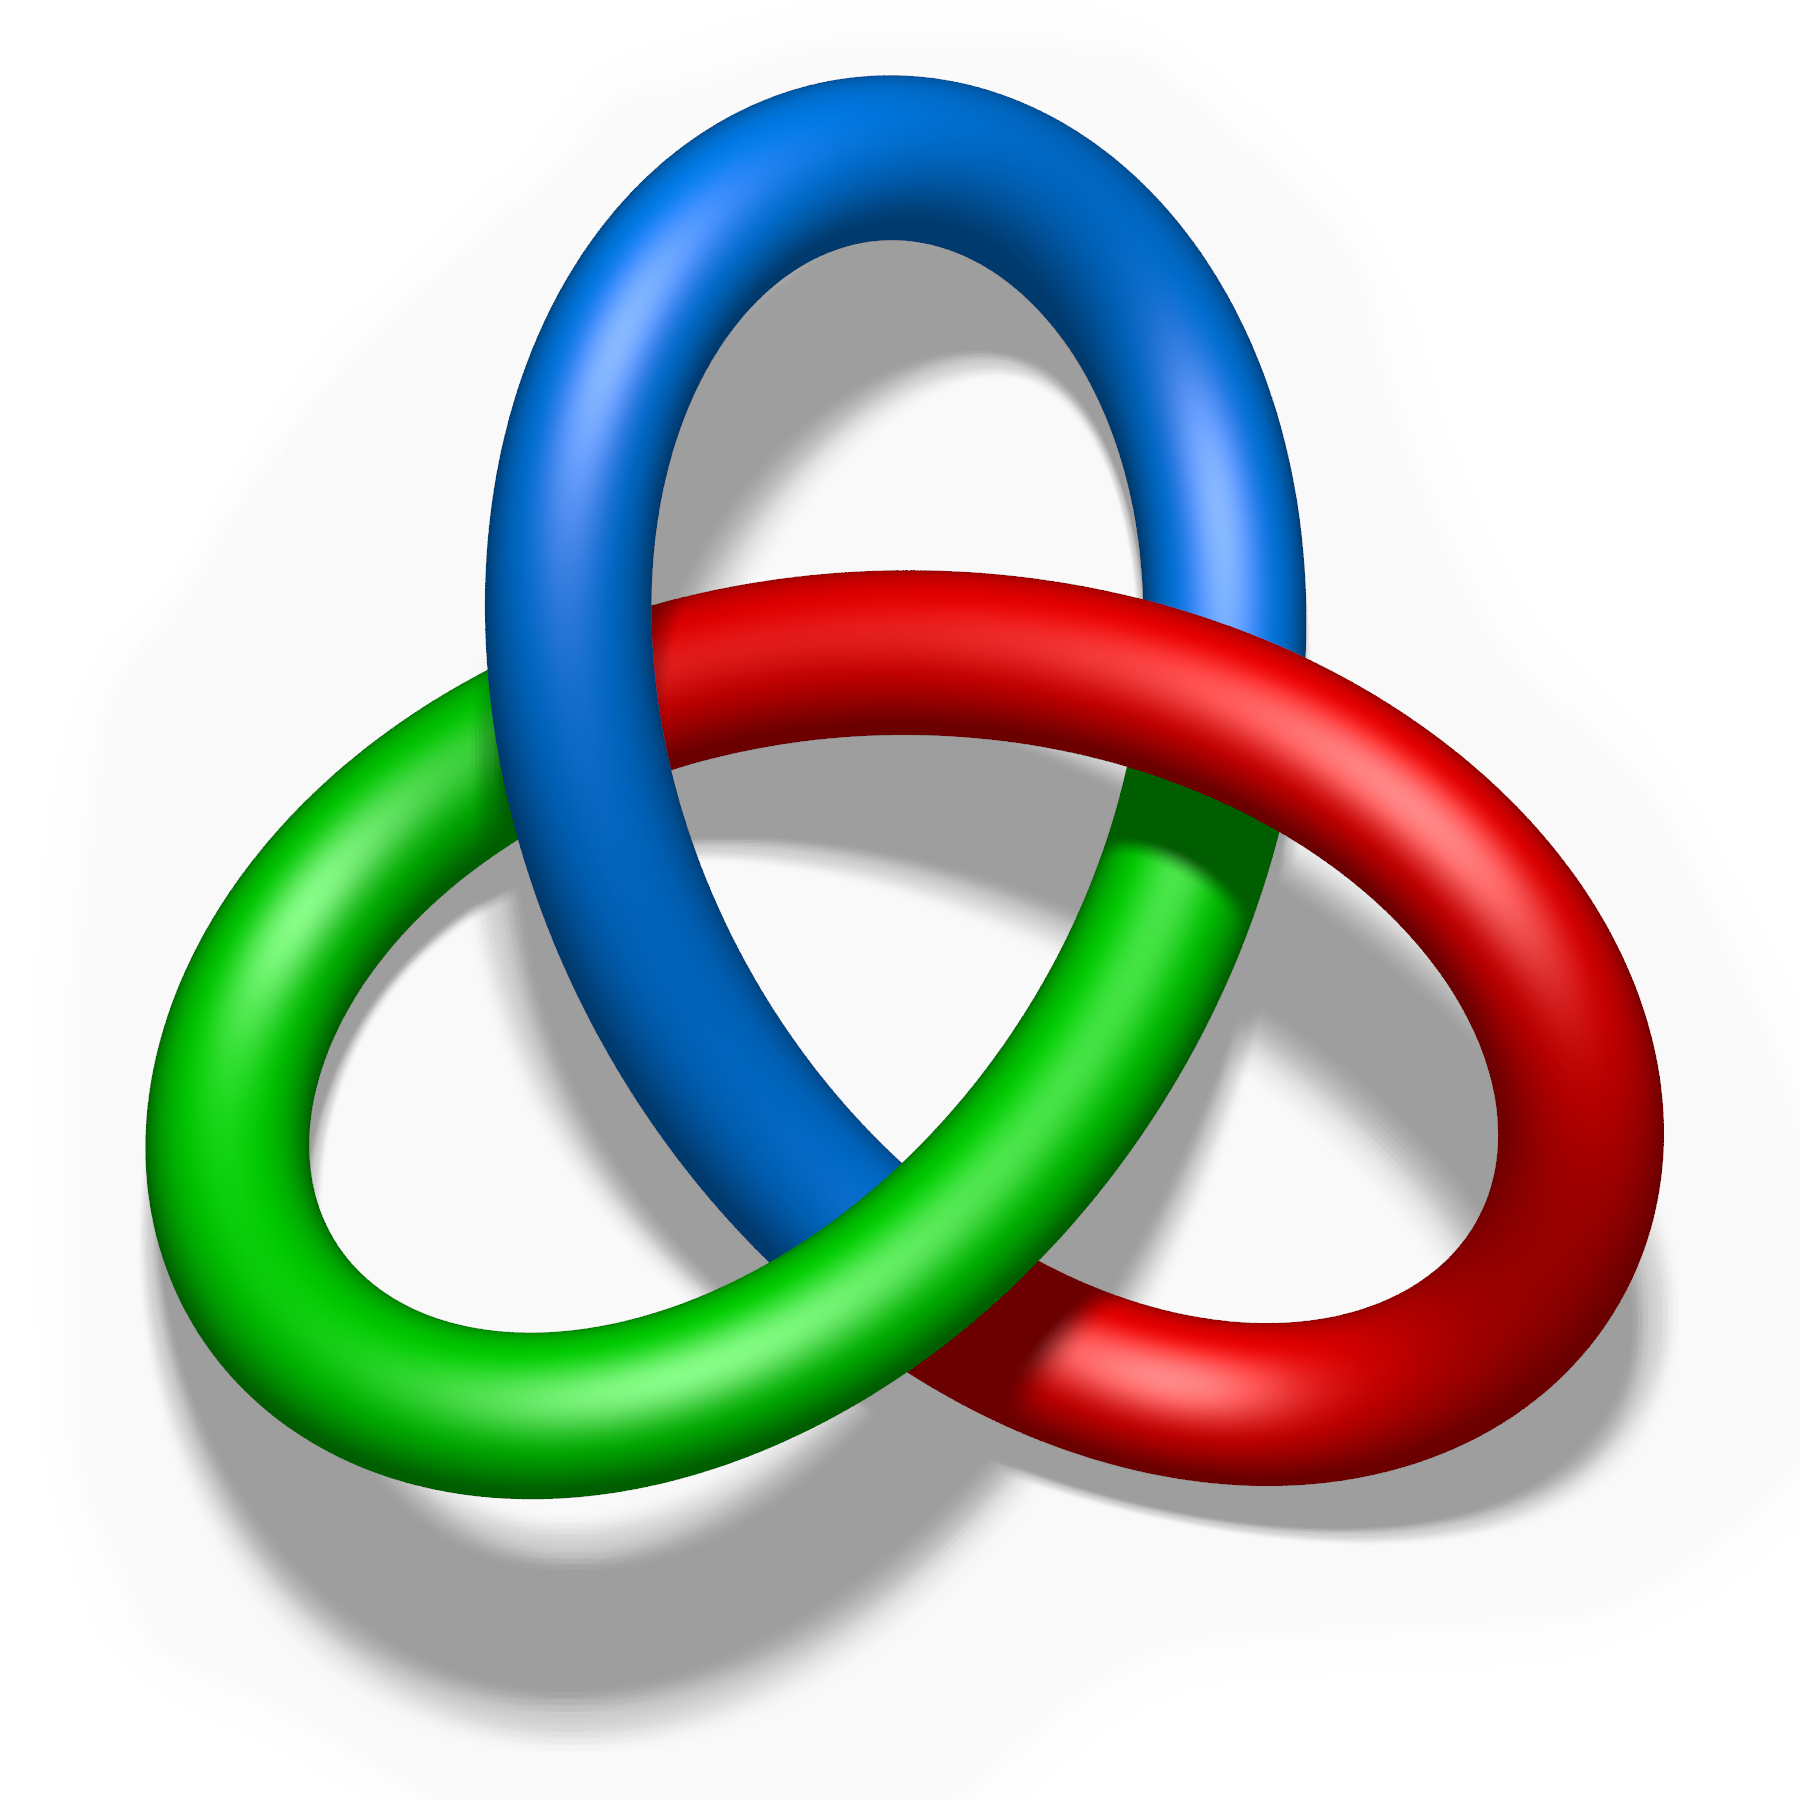
\includegraphics[width=2in,keepaspectratio]{tricoloring.png}};
      \end{tikzpicture}
      
    \end{frame}

    % https://tex.stackexchange.com/questions/506666/change-path-color-at-specified-points-to-tricolor-trefoil-knot
    \begin{frame}
      \begin{center}
      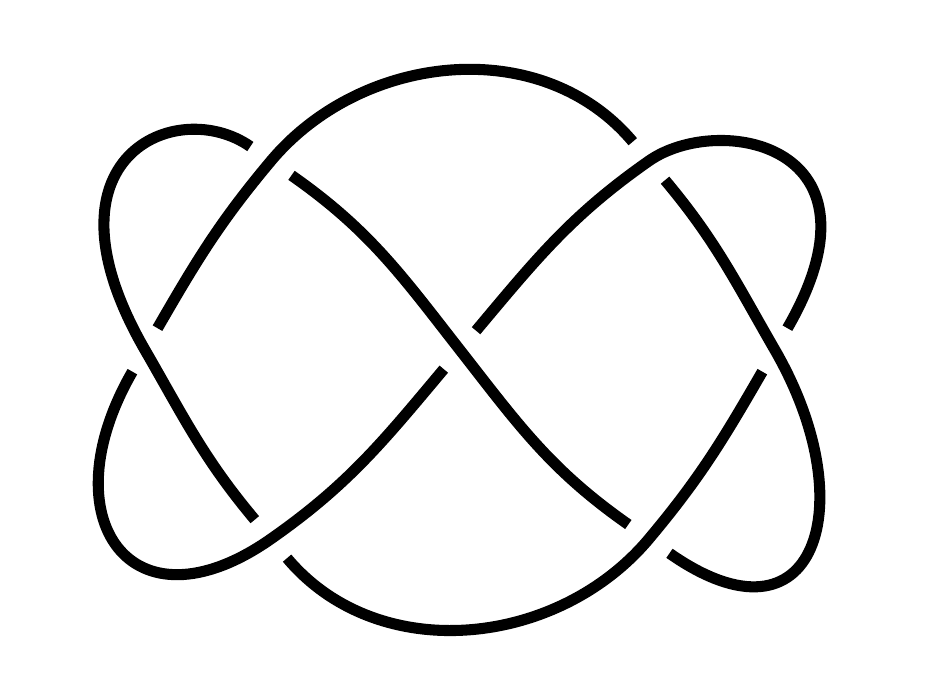
\begin{tikzpicture}[
        scale=4,
    every path/.style={thick, line width=4pt},
    every node/.style={knot crossing,inner sep=5pt}
]
\colorlet{rex}{black}
\colorlet{orx}{black}
    \colorlet{ylx}{black}

    \node (l) at (-1,0) {};
    \node (c) at (0,0) {};
    \node (r) at (1,0) {};
    \node (lu) at (-0.6,0.6) {};
    \node (lb) at (-0.6,-0.6) {};
    \node (ru) at (0.6,0.6) {};
    \node (rb) at (0.6,-0.6) {};

    \draw [orx] (lb)
        to [out=-50,in=-130] (rb.center)
        to [out=50,in=-120] (r)
    ;
    \draw [rex] (r)
        to [out=60,in=35,out looseness=2.5] (ru.center)
        to [out=-145,in=50] (c)
    ;
    \draw [rex] (c)
        to [out=-130,in=35] (lb.center)
        to [out=-145,in=-120,looseness=2] (l)
    ;
    \draw [orx] (l)
        to [out=60,in=-130] (lu.center)
        to [out=50,in=130] (ru)
    ;
    \draw [ylx] (ru)
        to [out=-50,in=120] (r.center)
        to [out=-60,in=-35,looseness=2] (rb)
    ;
    \draw [rex] (rb)
        to [out=145,in=-52] (c.center)
        to [out=128,in=-35] (lu)
    ;
    \draw [ylx] (lu)
        to [out=145,in=120,in looseness=2.5] (l.center)
        to [out=-60,in=130] (lb)
    ;
  \end{tikzpicture}
  \end{center}
\end{frame}

    \begin{frame}
      \begin{center}
      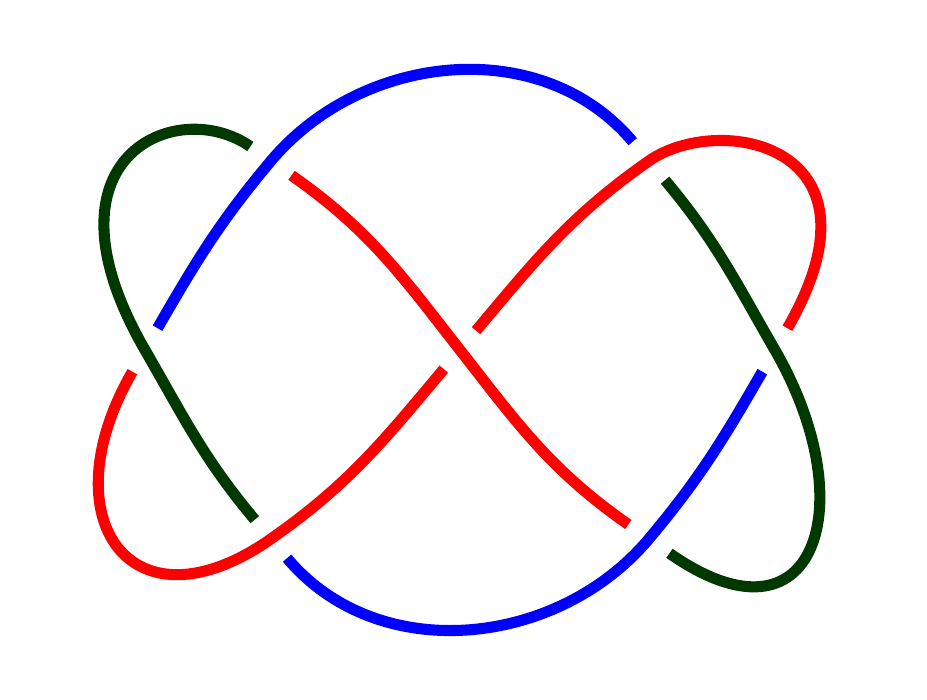
\begin{tikzpicture}[
        scale=4,
    every path/.style={thick, line width=4pt},
    every node/.style={knot crossing,inner sep=5pt}
]
    \colorlet{rex}{red}
    \colorlet{orx}{blue}
    \colorlet{ylx}{black!78!green}

    \node (l) at (-1,0) {};
    \node (c) at (0,0) {};
    \node (r) at (1,0) {};
    \node (lu) at (-0.6,0.6) {};
    \node (lb) at (-0.6,-0.6) {};
    \node (ru) at (0.6,0.6) {};
    \node (rb) at (0.6,-0.6) {};

    \draw [orx] (lb)
        to [out=-50,in=-130] (rb.center)
        to [out=50,in=-120] (r)
    ;
    \draw [rex] (r)
        to [out=60,in=35,out looseness=2.5] (ru.center)
        to [out=-145,in=50] (c)
    ;
    \draw [rex] (c)
        to [out=-130,in=35] (lb.center)
        to [out=-145,in=-120,looseness=2] (l)
    ;
    \draw [orx] (l)
        to [out=60,in=-130] (lu.center)
        to [out=50,in=130] (ru)
    ;
    \draw [ylx] (ru)
        to [out=-50,in=120] (r.center)
        to [out=-60,in=-35,looseness=2] (rb)
    ;
    \draw [rex] (rb)
        to [out=145,in=-52] (c.center)
        to [out=128,in=-35] (lu)
    ;
    \draw [ylx] (lu)
        to [out=145,in=120,in looseness=2.5] (l.center)
        to [out=-60,in=130] (lb)
    ;
  \end{tikzpicture}
  \end{center}
\end{frame}


%%%%%%%%%%%%%%%%%%%%%%%%%%%%%%%%%%%%%%%%%%%%%%%%%%%%%%%%%%%%%%%%
\begin{frame}
  \frametitle{Tricoloring Reidemeister Move II}

  \begin{center}
  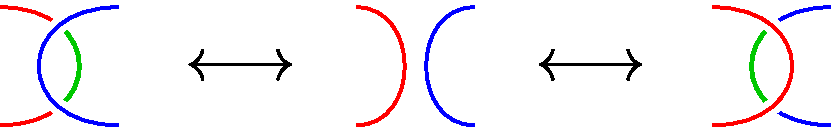
\includegraphics{r2-tricolor.pdf}
\end{center}
\end{frame}


%%%%%%%%%%%%%%%%%%%%%%%%%%%%%%%%%%%%%%%%%%%%%%%%%%%%%%%%%%%%%%%%
\begin{frame}
  \frametitle{Tricoloring Reidemeister Move III}

  \begin{center}
  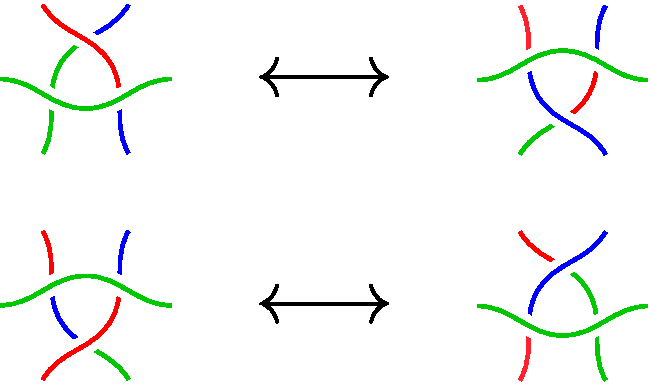
\includegraphics{r3-tricolor.pdf}
\end{center}
\end{frame}

\begin{frame}
  \begin{columns}
    \begin{column}{0.5\textwidth}
      \begin{center}
      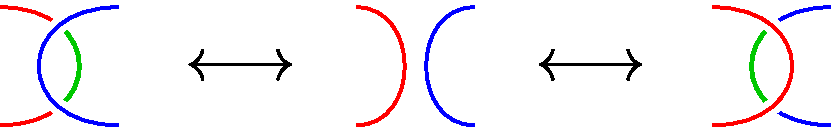
\includegraphics[scale=0.5]{r2-tricolor.pdf}
    \end{center}
    \vspace{0.001in}
    \begin{center}
      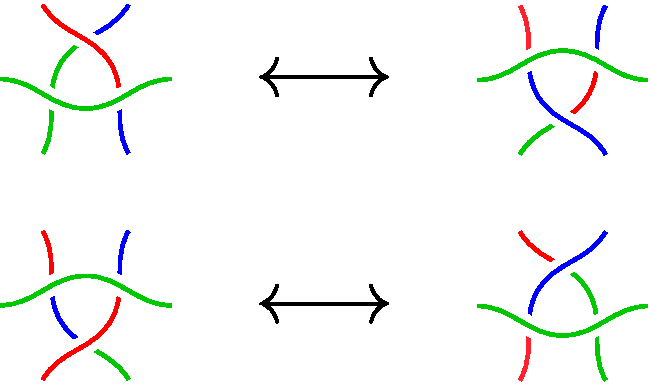
\includegraphics[scale=0.5]{r3-tricolor.pdf}
      \end{center}
    \end{column}
    \begin{column}{0.5\textwidth}
      \large
      A tricolorable diagram is \\
      \quad tricolorable after a move.
    \end{column}
  \end{columns}
  
\end{frame}

\begin{frame}
  \frametitle{How can we be sure a knot isn't the unknot?}

     \begin{tikzpicture}[
        scale=1.4,
    every path/.style={thick, line width=4pt},
    every node/.style={knot crossing,inner sep=5pt}
]
\alt<2>{\colorlet{rex}{blue}
\colorlet{orx}{red}
\colorlet{ylx}{black!78!green}}{
\colorlet{rex}{black}
\colorlet{orx}{black}
\colorlet{ylx}{black}}

    \node (l) at (-1,0) {};
    \node (c) at (0,0) {};
    \node (r) at (1,0) {};
    \node (lu) at (-0.6,0.6) {};
    \node (lb) at (-0.6,-0.6) {};
    \node (ru) at (0.6,0.6) {};
    \node (rb) at (0.6,-0.6) {};

    \draw [orx] (lb)
        to [out=-50,in=-130] (rb.center)
        to [out=50,in=-120] (r)
    ;
    \draw [rex] (r)
        to [out=60,in=35,out looseness=2.5] (ru.center)
        to [out=-145,in=50] (c)
    ;
    \draw [rex] (c)
        to [out=-130,in=35] (lb.center)
        to [out=-145,in=-120,looseness=2] (l)
    ;
    \draw [orx] (l)
        to [out=60,in=-130] (lu.center)
        to [out=50,in=130] (ru)
    ;
    \draw [ylx] (ru)
        to [out=-50,in=120] (r.center)
        to [out=-60,in=-35,looseness=2] (rb)
    ;
    \draw [rex] (rb)
        to [out=145,in=-52] (c.center)
        to [out=128,in=-35] (lu)
    ;
    \draw [ylx] (lu)
        to [out=145,in=120,in looseness=2.5] (l.center)
        to [out=-60,in=130] (lb)
    ;
  \end{tikzpicture}
  \raisebox{-0.1in}{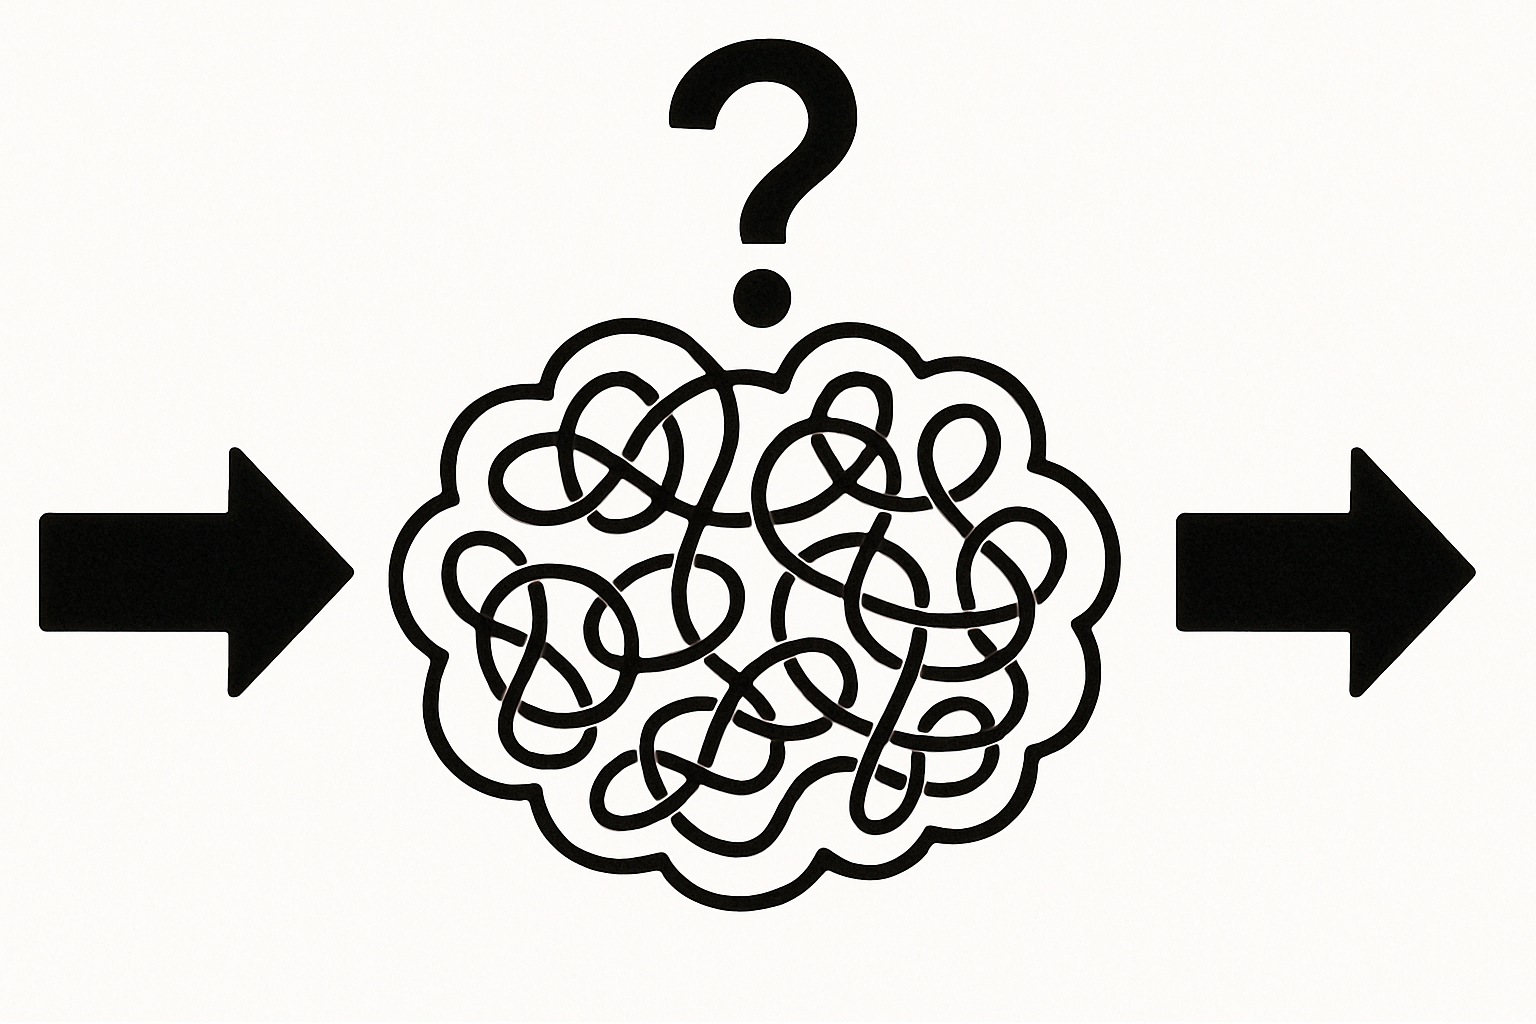
\includegraphics[width=2.5in]{knot-cloud.png}}
    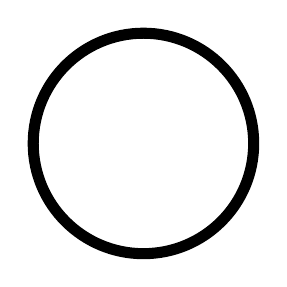
\begin{tikzpicture}[scale=1.4]
  \begin{knot}
    \strand[line width=4pt] (0,0) circle (1cm);
  \end{knot}
\end{tikzpicture}

\begin{center}\Large
\uncover<2>{\hspace{0.2in}tricolorable \hfill not tricolorable}
\end{center}

\end{frame}


\begin{frame}
  \frametitle{There are knots which aren't the unknot!}

  \begin{center}
     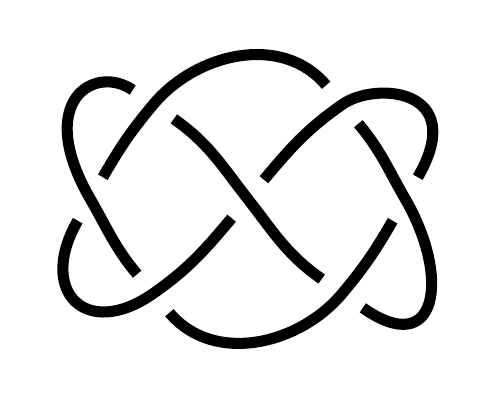
\begin{tikzpicture}[
        scale=2,
    every path/.style={thick, line width=4pt},
    every node/.style={knot crossing,inner sep=5pt}
]
\colorlet{rex}{black}
\colorlet{orx}{black}
\colorlet{ylx}{black}

    \node (l) at (-1,0) {};
    \node (c) at (0,0) {};
    \node (r) at (1,0) {};
    \node (lu) at (-0.6,0.6) {};
    \node (lb) at (-0.6,-0.6) {};
    \node (ru) at (0.6,0.6) {};
    \node (rb) at (0.6,-0.6) {};

    \draw [orx] (lb)
        to [out=-50,in=-130] (rb.center)
        to [out=50,in=-120] (r)
    ;
    \draw [rex] (r)
        to [out=60,in=35,out looseness=2.5] (ru.center)
        to [out=-145,in=50] (c)
    ;
    \draw [rex] (c)
        to [out=-130,in=35] (lb.center)
        to [out=-145,in=-120,looseness=2] (l)
    ;
    \draw [orx] (l)
        to [out=60,in=-130] (lu.center)
        to [out=50,in=130] (ru)
    ;
    \draw [ylx] (ru)
        to [out=-50,in=120] (r.center)
        to [out=-60,in=-35,looseness=2] (rb)
    ;
    \draw [rex] (rb)
        to [out=145,in=-52] (c.center)
        to [out=128,in=-35] (lu)
    ;
    \draw [ylx] (lu)
        to [out=145,in=120,in looseness=2.5] (l.center)
        to [out=-60,in=130] (lb)
    ;
  \end{tikzpicture}
  \hspace{0.01em}\raisebox{0.65in}{\scalebox{3}{$\neq$}}\hspace{0.5em}
    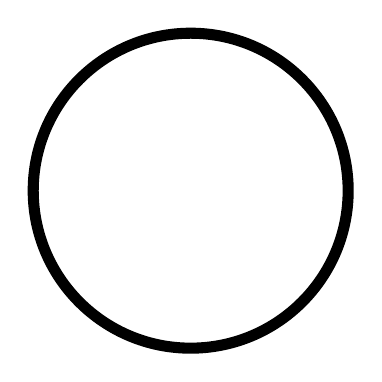
\begin{tikzpicture}[scale=2]
  \begin{knot}
    \strand[line width=4pt] (0,0) circle (1cm);
  \end{knot}
\end{tikzpicture}
\end{center}

\end{frame}

\begin{frame}
  \begin{center}
    
\includegraphics[height=2.2in,valign=c]{qr-trefoil.pdf}
    \hfill
    
\includegraphics[height=1.7in,valign=c]{tricoloring-trefoil.pdf}
    \hfill
  \end{center}

  \begin{center}\Large
    \textbf{\texttt{https://go.osu.edu/trefoil}}
  \end{center}
\end{frame}

\begin{frame}
  \frametitle{There are knots which aren't the unknot!}

  \begin{center}
    
\includegraphics[height=4cm]{tricoloring-trefoil.pdf}
    \hspace{0.01em}\raisebox{0.65in}{\scalebox{3}{$\neq$}}\hspace{0.5em}
    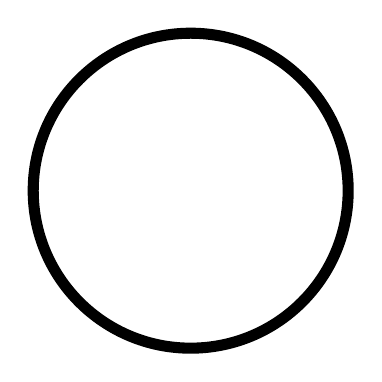
\begin{tikzpicture}[scale=2]
  \begin{knot}
    \strand[line width=4pt] (0,0) circle (1cm);
  \end{knot}
\end{tikzpicture}
\end{center}

\end{frame}


\begin{frame}
  \begin{center}
    
\includegraphics[height=2.2in,valign=c]{qr-granny-knot.pdf}
    \hfill
    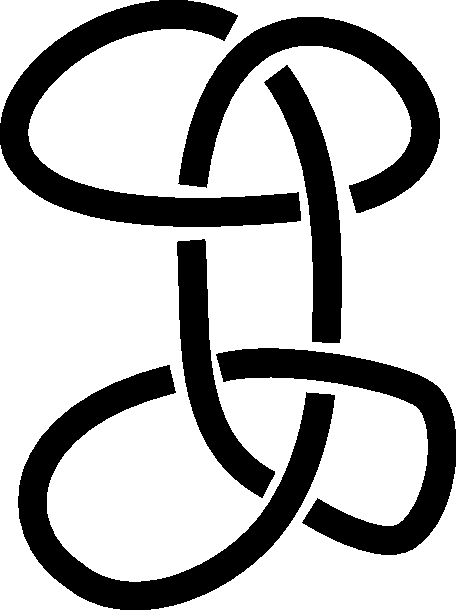
\includegraphics[height=2.2in,valign=c]{tricoloring-granny-knot.pdf}
    \hfill
  \end{center}

  \begin{center}\Large
    \textbf{\texttt{https://go.osu.edu/granny-knot}}
  \end{center}
\end{frame}

\begin{frame}
  \frametitle{There are knots which aren't the unknot!}

  \begin{center}
    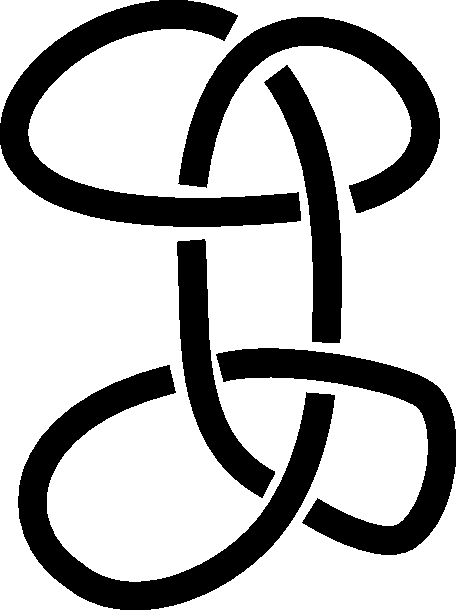
\includegraphics[height=4cm]{tricoloring-granny-knot.pdf}
    \hspace{0.01em}\raisebox{0.65in}{\scalebox{3}{$\neq$}}\hspace{0.5em}
    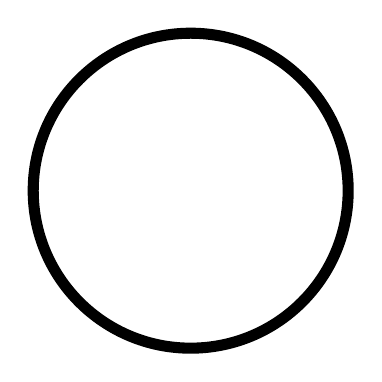
\begin{tikzpicture}[scale=2]
  \begin{knot}
    \strand[line width=4pt] (0,0) circle (1cm);
  \end{knot}
\end{tikzpicture}
\end{center}

\end{frame}

\begin{frame}
  \begin{center}
    
\includegraphics[height=2.2in,valign=c]{qr-figure-eight.pdf}
    \hfill
    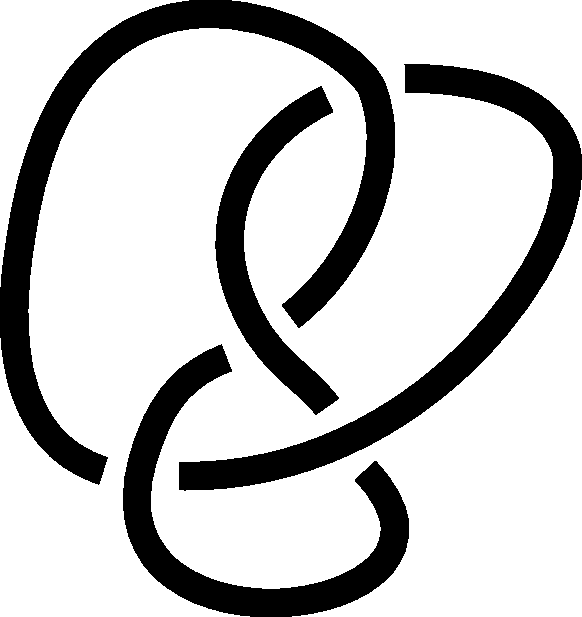
\includegraphics[height=2.2in,valign=c]{tricoloring-figure-eight.pdf}
    \hfill
  \end{center}

  \begin{center}\Large
    \textbf{\texttt{https://go.osu.edu/figure-eight}}
  \end{center}
\end{frame}

\begin{frame}
  \frametitle{Is the figure eight knot not the unknot?}
  \begin{center}
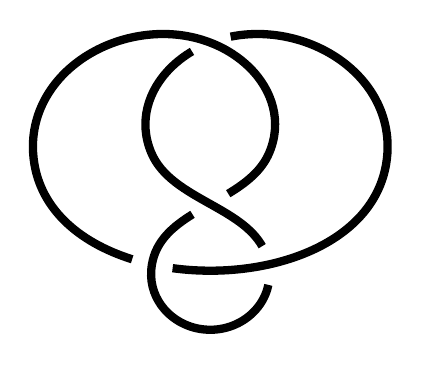
\begin{tikzpicture}[use Hobby shortcut,scale=1.5]
\path[spath/save=figure8]
([closed]0,0) .. (1.5,1) .. (.5,2) ..
(-.5,1) .. (.5,0) .. (0,-.5) .. (-.5,0) ..
(.5,1) .. (-.5,2) .. (-1.5,1) .. (0,0);
\tikzset{
  spath component/.style={
    line width=3pt,
    draw,
  },
  spath/knot={figure8}{15pt}{1,3,...,7}
}
\path (0,-.7);
\end{tikzpicture}
  \hspace{1em}\raisebox{0.65in}{\scalebox{3}{$\stackrel{?}{\neq}$}}\hspace{1em}
    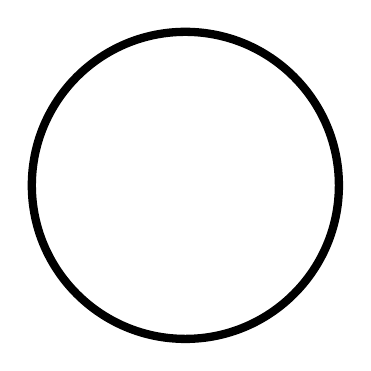
\begin{tikzpicture}[scale=1.5]
  \begin{knot}
    \strand[line width=3pt] (0,0) circle (1.3cm);
  \end{knot}
\end{tikzpicture}
\end{center}

\end{frame}

\begin{frame}
  \frametitle{Conway Polynomial}
  \Large
  
  For a knot $K$, \\
  \quad we define $\nabla(K)$, \\
  \quad\quad the Conway polynomial of $K$, \\
  \quad which doesn't depend on the diagram.
  
\end{frame}

% define a mid-strand arrow style
\tikzset{
  mid arrow/.style={
    decoration={markings,
      mark=at position 0.75 with {\arrow{>}}
    },
    postaction={decorate}
  }
}

\newcommand{\kpos}{%
  \tikz[baseline=-0.5ex, scale=0.35]{
    % dotted circle
    \draw[dotted] (0,0) circle (1);
    % draw crossing
    \begin{knot}[clip width=8, background color=white]
      \strand (-0.7,-0.7) to[out=45,in=225] (0.7,0.7);
      \strand[overcross] (-0.7, 0.7) to[out=315,in=135] (0.7,-0.7);
    \end{knot}
    \draw[->] (0.5,0.5) to[out=45,in=225] (0.6,0.6);
    \draw[->] (-0.5, 0.5) -- (-0.6,0.6);
  }%
}

\newcommand{\kneg}{%
  \tikz[baseline=-0.5ex, scale=0.35]{
    % dotted circle
    \draw[dotted] (0,0) circle (1);
    % draw crossing
    \begin{knot}[clip width=8, background color=white]
      \strand (-0.7, 0.7) to[out=315,in=135] (0.7,-0.7);
      \strand[overcross] (-0.7,-0.7) to[out=45,in=225] (0.7,0.7);
    \end{knot}
    \draw[->] (0.5,0.5) to[out=45,in=225] (0.6,0.6);
    \draw[->] (-0.5, 0.5) -- (-0.6,0.6);
  }%
}

% Smoothing in a dotted circle
\newcommand{\ksmooth}{%
  \tikz[baseline=-0.5ex, scale=0.35]{
    % dotted circle
    \draw[dotted] (0,0) circle (1);
    % draw smoothing arcs
    \draw[->] (-0.7, -0.7) to[out=45,in=315] (-0.7, 0.7);
    \draw[->] (0.7, -0.7) to[out=135,in=225] (0.7, 0.7);
  }%
}

% Smoothing in a dotted circle
\newcommand{\unknot}{%
  \tikz[baseline=-0.5ex, scale=0.35]{
    \draw[line width=1.2pt] (0,0) circle (0.7);
  }%
}

\begin{frame}
  \frametitle{Skein relations}
  \large
  \begin{center}
    $\nabla(\unknot) = 1$ and $\nabla(\kpos) = \nabla(\kneg) + x \nabla(\ksmooth)$.
  \end{center}

  \vfill
  
  Then $\nabla(\text{trefoil}) = 1 + x^2$ and $\nabla(\text{figure eight}) = 1 - x^2$.

  \vfill

  So $\text{trefoil} \neq \text{figure eight}$ and $\text{figure eight} \neq \text{unknot}$.
\end{frame}

\begin{frame}
  \huge

  \begin{center}
    \scalebox{2.5}{\textbf{Tangles}}
  \end{center}
\end{frame}

\begin{frame}
  \frametitle{What is\ldots a \textbf{tangle}?}

  \begin{center}
      \displaytangle{\tangletwist{\tanglerotate{\tangletwist{\tangleone}}}}
    \hfill
      \displaytangle{\tangletwist{\tanglerotate{\tangletwist{\tangletwist{\tangleone}}}}}
      \hfill
      \displaytangle{\tanglerotate{\tangletwist{\tangletwist{\tanglerotate{\tangletwist{\tangleone}}}}}}
  \end{center}

\end{frame}

\newcommand{\rotategeneric}{
    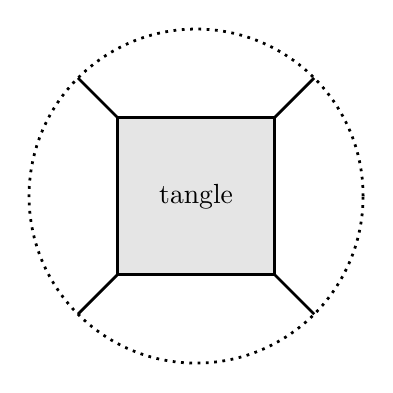
\begin{tikzpicture}[line width=1pt]

  % The central square
  \draw[fill=white!90!black] (0,0) rectangle (2,2);

  % Label T at the center
  \node at (1,1) {tangle};

  % Four strands from the corners
  \draw (0,0) -- ++(-0.5,-0.5);
  \draw (2,0) -- ++(0.5,-0.5);
  \draw (2,2) -- ++(0.5,0.5);
  \draw (0,2) -- ++(-0.5,0.5);

  \draw[dotted] (1,1) circle (2.12132034355964);
  
\end{tikzpicture}
\raisebox{0.7in}{\scalebox{2}{$\xmapsto{R}$}}
  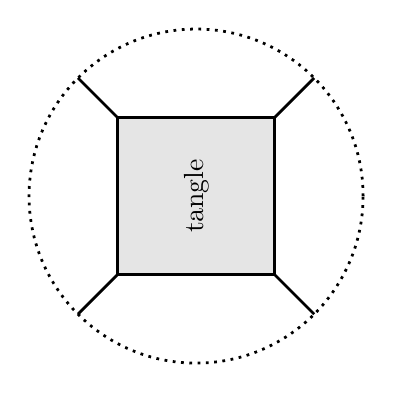
\begin{tikzpicture}[line width=1pt]

    \begin{scope}[rotate around={90:(1,1)}]
      % The central square
      \draw[fill=white!90!black] (0,0) rectangle (2,2);

      % Label T at the center
      \node[rotate=90] at (1,1) {tangle};
    \end{scope}
    
  % Four strands from the corners
  \draw (0,0) -- ++(-0.5,-0.5);
  \draw (2,0) -- ++(0.5,-0.5);
  \draw (2,2) -- ++(0.5,0.5);
  \draw (0,2) -- ++(-0.5,0.5);

  \draw[dotted] (1,1) circle (2.12132034355964);
  
\end{tikzpicture}
}

%%%%%%%%%%%%%%%%%%%%%%%%%%%%%%%%%%%%%%%%%%%%%%%%%%%%%%%%%%%%%%%%
\begin{frame}
  \frametitle{Operations on Tangles: Rotate}

  \begin{center}
    \rotategeneric
\end{center}
  
\end{frame}

\newcommand{\generictangle}{\tangletwist{\tanglerotate{\tangletwist{\tangletwist{\tangleone}}}}}

\begin{frame}
  \frametitle{Operations on Tangles: Rotate}

  \raisebox{0.65in}{\scalebox{3}{$R($}} \displaytangle{\generictangle} \raisebox{0.65in}{\scalebox{3}{$) = $}} \displaytangle{\tanglerotate{\generictangle}}
\end{frame}

\newcommand{\twistgeneric}{
    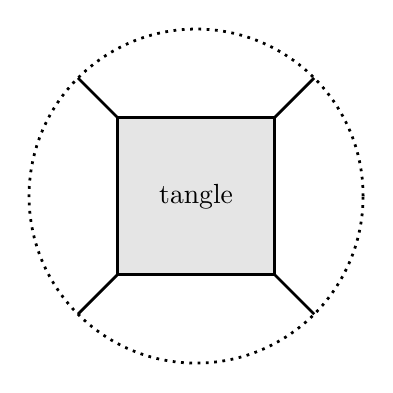
\begin{tikzpicture}[line width=1pt]

  % The central square
  \draw[fill=white!90!black] (0,0) rectangle (2,2);

  % Label T at the center
  \node at (1,1) {tangle};

  % Four strands from the corners
  \draw (0,0) -- ++(-0.5,-0.5);
  \draw (2,0) -- ++(0.5,-0.5);
  \draw (2,2) -- ++(0.5,0.5);
  \draw (0,2) -- ++(-0.5,0.5);

  \draw[dotted] (1,1) circle (2.12132034355964);
  
\end{tikzpicture}
\raisebox{0.7in}{\scalebox{2}{$\xmapsto{T}$}}
  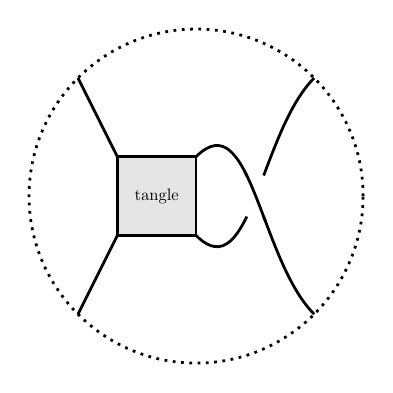
\begin{tikzpicture}[line width=1pt]

    \begin{scope}[yshift=0.5cm]
    \begin{scope}[scale=0.5,rotate around={90:(1,1)}]
      % The central square
      \draw[fill=white!90!black] (0,0) rectangle (2,2);

      % Label T at the center
      \node[scale=0.6] at (1,1) {tangle};
    \end{scope}
    \end{scope}
    
  % Four strands from the corners
  \draw (0,0.5) -- ++(-0.5,-1);
  \draw (0,1.5) -- ++(-0.5,1);

  \begin{knot}[clip width=5, clip radius=8pt]
    \strand (1,1.5) to[out=45,in=135] (2.5,-0.5);
    \strand (1,0.5) to[out=-45,in=-135] (2.5,2.5);
  \end{knot}

  \draw[dotted] (1,1) circle (2.12132034355964);
  
\end{tikzpicture}
}

%%%%%%%%%%%%%%%%%%%%%%%%%%%%%%%%%%%%%%%%%%%%%%%%%%%%%%%%%%%%%%%%
\begin{frame}
  \frametitle{Operations on Tangles: Twist}

  \begin{center}
    \twistgeneric
  \end{center}

\end{frame}

\begin{frame}
  \frametitle{Operations on Tangles: Twist}

  \raisebox{0.65in}{\scalebox{3}{$T($}} \displaytangle{\generictangle} \raisebox{0.65in}{\scalebox{3}{$) = $}} \displaytangle{\tangletwist{\generictangle}}
\end{frame}

\begin{frame}
  \frametitle{Rotate and Twist, $R$ and $T$.}
  \begin{center}
    \scalebox{0.6}{\rotategeneric} \raisebox{0.4in}{and} \scalebox{0.6}{\twistgeneric}
  \end{center}

  We can record a sequence of operations as a string of $R$s and $T$s.
\end{frame}
  
\begin{frame}
    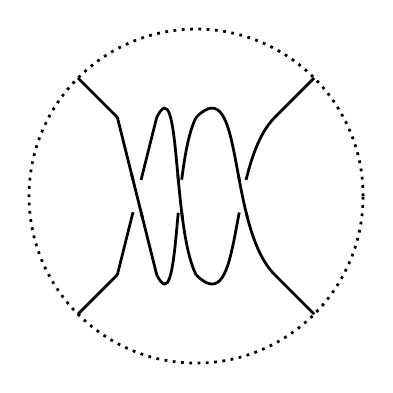
\begin{tikzpicture}[line width=1pt]

      % \tangletwist{\tanglerotate{\tangletwist{\tangletwist{\tangleT}}}}
      \tangletwist{\tangletwist{\tangleone}}
      %\tangletwist{\tangleT}
    
      \draw (-1,-1) -- (-1.5,-1.5);
      \draw ( 1,-1) -- ( 1.5,-1.5);
      \draw (-1, 1) -- (-1.5, 1.5);
      \draw ( 1, 1) -- ( 1.5, 1.5);

  \draw[dotted] (0,0) circle (2.12132034355964);
  
\end{tikzpicture}

\end{frame}

\end{document}
